\section{Introducción}

\subsection{Consigna e interpretación}
La Consigna 6 de la actividad evaluativa de la Unidad 6 pide:
\begin{quote}
\emph{``Diseñar y calcular una fuente de alimentación con un regulador lineal integrado LM7805. Se dispone de una fuente primaria de \SI{25}{\volt} dc. A los fines de mejorar la regulación del voltaje de línea es necesario un rango de $V_{in} = \SI{8}{}$--$\SI{12}{\volt}$. Incluir en el diseño una etapa que cumpla con este objetivo. Verificar mediante simulación la regulación de línea para $V_{in} = \SI{25}{\volt}$ y $V_{in} = \SI{10}{\volt}$. Seleccionar transistor, verificar punto de operación según SOA e incluir eventual cálculo de disipador. Obtener todos los parámetros de calidad de fuentes de alimentación.''}
\end{quote}

En el enunciado, $V_{in}$ es la tensión de entrada del regulador: el rango de \SI{8}{\volt} a \SI{12}{\volt} es el que la hoja de datos del LM7805 usa para especificar su mejor regulación de línea. Por eso la verificación pedida se interpreta como la comparación entre dos situaciones: el LM7805 conectado directo a la fuente primaria ($V_{in} = \SI{25}{\volt}$) y el LM7805 alimentado a través de la etapa prereguladora, que lleva su entrada a unos \SI{10}{\volt}. Para cubrir también la otra lectura posible, se simula el caso en que la propia fuente primaria baja a \SI{10}{\volt} (Sección~\ref{sec:linea}).

\subsection{Especificaciones de diseño}
La consigna no fija la corriente de carga. Se adopta $I_{L,\max} = \SI{0,5}{\ampere}$, que es la corriente con la que la hoja de datos especifica las características eléctricas del regulador~\cite{ua78}, y $I_{L,\min} = 0$, como establece el apunte para la regulación de carga~\cite[Sec.~6-6-3b]{ap2}. La Tabla~\ref{tab:especificaciones} resume el resto de los datos de partida. La variación de $\pm\SI{10}{\percent}$ de la fuente primaria es la que el apunte toma para la regulación de red~\cite[Sec.~6-6-3a]{ap2}, y la temperatura ambiente máxima y la de juntura de diseño son las del Ejemplo~9 del apunte~\cite[Sec.~6-8-3b]{ap2}. El rizado de prueba de \SI{2}{\volt} pico a pico a \SI{100}{\hertz} representa una fuente primaria obtenida con un rectificador de onda completa de \SI{50}{\hertz}; se usa solo para medir el rechazo de rizado.

\begin{table}[!htb]
\centering
\caption{Especificaciones adoptadas para el diseño.}
\label{tab:especificaciones}
\begin{tabular}{lc}
\toprule
\textbf{Parámetro} & \textbf{Valor} \\
\midrule
Fuente primaria $\Vp$ & \SI{25}{\volt} $\pm\SI{10}{\percent}$ (\SI{22,5}{} a \SI{27,5}{\volt}) \\
Tensión de salida $V_O$ & \SI{5}{\volt} (LM7805) \\
Corriente de carga $I_L$ & \SI{0}{} a \SI{0,5}{\ampere} \\
Entrada del regulador $\Vireg$ & \SI{8}{} a \SI{12}{\volt} \\
Temperatura ambiente máxima $T_a$ & \SI{40}{\celsius} \\
Temperatura de juntura de diseño $T_J$ & \SI{100}{\celsius} \\
Rizado de prueba en $\Vp$ & \SI{2}{\volt} pico a pico, \SI{100}{\hertz} \\
\bottomrule
\end{tabular}
\end{table}

\subsection{El regulador LM7805}
Los reguladores de la familia 78XX integran en un mismo chip el elemento serie (un par Darlington), una referencia de tensión, la red de muestreo, el amplificador de error y tres protecciones: limitación de corriente, protección de área segura, que reduce la corriente disponible cuando crece la diferencia $V_I - V_O$, y corte por temperatura~\cite[Sec.~6-9-1 y 6-9-2]{ap3}, \cite[Sec.~15-8.3]{coughlin}. La Fig.~\ref{fig:bloques_7805} muestra el diagrama en bloques y la Tabla~\ref{tab:datasheet_7805} los datos de la hoja de datos que se usan en este trabajo.

\begin{figure}[!htb]
\centering
\resizebox{\columnwidth}{!}{%
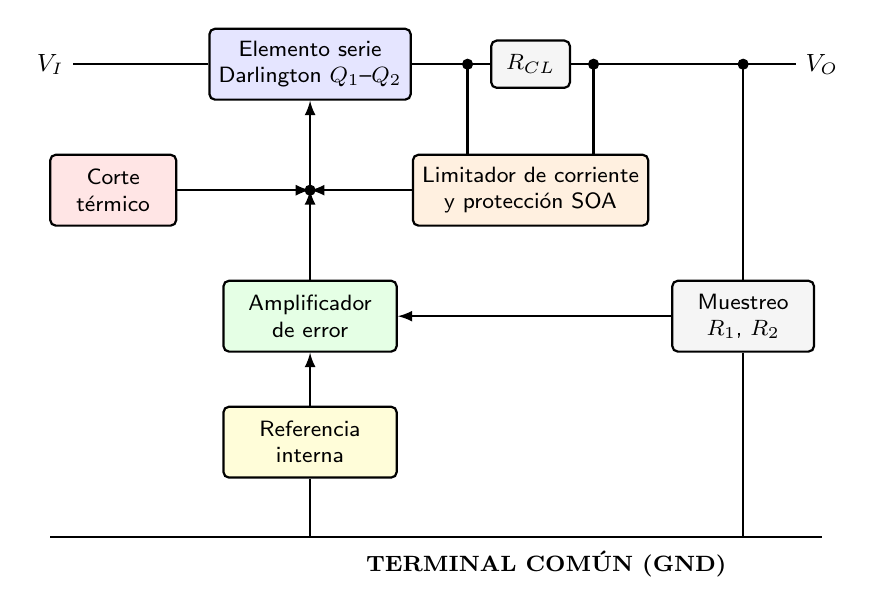
\begin{tikzpicture}[
    block/.style={draw, thick, rectangle, rounded corners=2pt, minimum height=0.9cm, align=center, font=\footnotesize\sffamily, fill=gray!8},
    line/.style={thick, -latex}
]
    % camino de potencia
    \node[font=\small] (vin) at (-0.9, 3.4) {$V_I$};
    \node[font=\small] (vout) at (8.9, 3.4) {$V_O$};
    \node[block, fill=blue!10, minimum width=2.4cm] (pass) at (2.4, 3.4) {Elemento serie\\Darlington $Q_1$--$Q_2$};
    \node[block, minimum width=1.0cm, minimum height=0.6cm] (rcl) at (5.2, 3.4) {$R_{CL}$};
    \draw[thick] (vin) -- (pass.west);
    \draw[thick] (pass.east) -- (rcl.west);
    \draw[thick] (rcl.east) -- (vout);
    % nodo de excitacion de base
    \coordinate (J) at (2.4, 1.8);
    \draw[line] (J) -- (pass.south);
    \filldraw (J) circle (1.8pt);
    % protecciones
    \node[block, fill=red!10, minimum width=1.6cm] (term) at (-0.1, 1.8) {Corte\\térmico};
    \draw[line] (term.east) -- (J);
    \node[block, fill=orange!12, minimum width=2.9cm] (lim) at (5.2, 1.8) {Limitador de corriente\\y protección SOA};
    \draw[line] (lim.west) -- (J);
    \filldraw (4.4, 3.4) circle (1.8pt);
    \filldraw (6.0, 3.4) circle (1.8pt);
    \draw[thick] (4.4, 3.4) -- (4.4, 2.25);
    \draw[thick] (6.0, 3.4) -- (6.0, 2.25);
    % lazo de regulacion
    \node[block, fill=green!10, minimum width=2.2cm] (amp) at (2.4, 0.2) {Amplificador\\de error};
    \draw[line] (amp.north) -- (J);
    \node[block, fill=yellow!15, minimum width=2.2cm] (ref) at (2.4, -1.4) {Referencia\\interna};
    \draw[line] (ref.north) -- (amp.south);
    \node[block, minimum width=1.8cm] (samp) at (7.9, 0.2) {Muestreo\\$R_1$, $R_2$};
    \filldraw (7.9, 3.4) circle (1.8pt);
    \draw[thick] (7.9, 3.4) -- (samp.north);
    \draw[line] (samp.west) -- (amp.east);
    % masa
    \draw[thick] (-0.9, -2.6) -- (8.9, -2.6);
    \draw[thick] (ref.south) -- (2.4, -2.6);
    \draw[thick] (samp.south) -- (7.9, -2.6);
    \node[font=\footnotesize\bfseries] at (5.4, -2.95) {TERMINAL COMÚN (GND)};
\end{tikzpicture}%
}
\caption{Diagrama en bloques del regulador LM7805 (adaptado de \cite[Fig.~6-55 a 6-57]{ap3}).}
\label{fig:bloques_7805}
\end{figure}

\begin{table}[!htb]
\centering
\caption{Características del $\mu$A7805C a $T_J = \SI{25}{\celsius}$, $V_I = \SI{10}{\volt}$ e $I_O = \SI{500}{\milli\ampere}$, salvo indicación~\cite{ua78}.}
\label{tab:datasheet_7805}
\footnotesize
\setlength{\tabcolsep}{3.5pt}
\begin{tabular}{@{}>{\raggedright}p{3.9cm}ccc@{}}
\toprule
\textbf{Parámetro y condición} & \textbf{Mín.} & \textbf{Típ.} & \textbf{Máx.} \\
\midrule
Tensión de salida, $I_O = \SI{5}{\milli\ampere}$ a \SI{1}{\ampere}, $V_I = \SI{7}{}$ a \SI{20}{\volt} & \SI{4,8}{\volt} & \SI{5}{\volt} & \SI{5,2}{\volt} \\
Regulación de línea, $V_I = \SI{7}{}$ a \SI{25}{\volt} & -- & \SI{3}{\milli\volt} & \SI{100}{\milli\volt} \\
Regulación de línea, $V_I = \SI{8}{}$ a \SI{12}{\volt} & -- & \SI{1}{\milli\volt} & \SI{50}{\milli\volt} \\
Rechazo de rizado, $V_I = \SI{8}{}$ a \SI{12}{\volt}, \SI{120}{\hertz} & \SI{62}{\deci\bel} & \SI{78}{\deci\bel} & -- \\
Regulación de carga, $I_O = \SI{5}{\milli\ampere}$ a \SI{1,5}{\ampere} & -- & \SI{15}{\milli\volt} & \SI{100}{\milli\volt} \\
Regulación de carga, $I_O = \SI{250}{}$ a \SI{750}{\milli\ampere} & -- & \SI{5}{\milli\volt} & \SI{50}{\milli\volt} \\
Resistencia de salida, $f = \SI{1}{\kilo\hertz}$ & -- & \SI{0,017}{\ohm} & -- \\
Coef.\ de temperatura, $I_O = \SI{5}{\milli\ampere}$ & -- & \SI{-1,1}{\milli\volt\per\celsius} & -- \\
Tensión de \emph{dropout}, $I_O = \SI{1}{\ampere}$ & -- & \SI{2}{\volt} & -- \\
Corriente de polarización & -- & \SI{4,2}{\milli\ampere} & \SI{8}{\milli\ampere} \\
Corriente de cortocircuito & -- & \SI{750}{\milli\ampere} & -- \\
Corriente de pico & -- & \SI{2,2}{\ampere} & -- \\
Tensión de entrada recomendada & \SI{7}{\volt} & -- & \SI{25}{\volt} \\
$R_{\theta JP}$, TO-220, juntura a aleta & -- & \SI{3}{\celsius\per\watt} & -- \\
\bottomrule
\end{tabular}
\end{table}

\subsection{Por qué conviene una entrada de \SI{8}{} a \SI{12}{\volt}}
La hoja de datos da dos valores de regulación de línea. Para $V_I$ entre \SI{7}{} y \SI{25}{\volt} la salida cambia \SI{3}{\milli\volt} típicos, y si la entrada se limita a la zona central, de \SI{8}{} a \SI{12}{\volt}, el cambio baja a \SI{1}{\milli\volt}~\cite[Sec.~6-9-3]{ap3}. Además:
\begin{itemize}
    \item El límite inferior surge del margen que necesita el regulador para que su elemento serie no salga de la zona activa: $V_{I,\min} = V_O + \text{margen} = \SI{5}{\volt} + \SI{3}{\volt} = \SI{8}{\volt}$~\cite[Ec.~15-8 y Sec.~15-9.2]{coughlin}. Con \SI{8}{\volt} queda \SI{1}{\volt} por encima del \emph{dropout} de \SI{2}{\volt}.
    \item Conectado directo a \SI{25}{\volt}, el LM7805 trabaja en el límite de su tensión de entrada recomendada y debe disipar $(25 - 5)\,\si{\volt} \times \SI{0,5}{\ampere} = \SI{10}{\watt}$. Con la entrada en unos \SI{10}{\volt}, la disipación baja a unos \SI{2,5}{\watt} y el resto de la caída la toma un transistor externo, más fácil de refrigerar.
\end{itemize}
